\documentclass{beamer}
\usepackage{polski}
\usepackage[utf8]{inputenc}

\usetheme{Frankfurt}

\mode<presentation>

\definecolor{polyured}{RGB}{50, 89, 40}% PMS 194C RGB #A02337
\definecolor{polyugrey}{RGB}{128,130,133}% PMS Cool Gray 10C #808285
\definecolor{polyugold}{RGB}{145,107,74}% PMS 875C RGB #916B4A
\definecolor{polyusilver}{RGB}{143,143,140}% PMS 877C RGB #8F8F8C
\definecolor{polyuorange}{RGB}{255,102,0}
\definecolor{polyuyellow}{RGB}{255,255,204}
\definecolor{polyuseventyfivered}{RGB}{153,15,61}% CMYK: 0,90,60,40
\definecolor{polyuseventyfivegrey}{RGB}{102,102,102}% CMYK: 0,0,0,60
\definecolor{polyuseventyfivegold}{RGB}{230,166,89}% Pantone 722C or CMYK: 10,35,65,0
\definecolor{polyuseventyfivegoldsecond}{RGB}{230,166,89}% Pantone 874C
\definecolor{polyublue}{RGB}{0,140,215} % COMP
\definecolor{polyuicyblue}{RGB}{83,195,241} % COMP
\definecolor{polyugreen}{RGB}{143,195,32} % COMP

\setbeamercolor{normal text}{fg=black,bg=white}
\setbeamercolor{alerted text}{fg=polyured}
\setbeamercolor{example text}{fg=polyured}

\setbeamercolor{background canvas}{parent=normal text}
\setbeamercolor{background}{parent=background canvas}

\setbeamercolor{structure}{fg=polyured,bg=white}

\setbeamercolor{palette primary}{fg=white,bg=polyured}
\setbeamercolor{palette secondary}{fg=white,bg=polyured!75}
\setbeamercolor{palette tertiary}{fg=white,bg=polyured!85}
\setbeamercolor{palette quaternary}{fg=white,bg=polyured}

\setbeamercolor{titlelike}{parent=palette primary}

\setbeamercolor{block title}{fg=white,bg=polyured}
\setbeamercolor{block title alerted}{use=alerted text,fg=white,bg=alerted text.fg}
\setbeamercolor{block title example}{use=example text,fg=white,bg=example text.fg}

\setbeamercolor{block body}{parent=normal text,use=block title,bg=block title.bg!15!bg}
\setbeamercolor{block body alerted}{parent=normal text,use=block title alerted,bg=block title alerted.bg!15!bg}
\setbeamercolor{block body example}{parent=normal text,use=block title example,bg=block title example.bg!15!bg}

\setbeamercolor{sidebar}{bg=polyured}

\setbeamercolor{palette sidebar primary}{fg=black!50}
\setbeamercolor{palette sidebar secondary}{fg=white!75}
\setbeamercolor{palette sidebar tertiary}{fg=white!75}
\setbeamercolor{palette sidebar quaternary}{fg=white}

\setbeamercolor*{separation line}{}
\setbeamercolor*{fine separation line}{}

\mode
<all>
\setbeamercovered{transparent}
\title[Realizacja frontalnego solwera MES]{Realizacja frontalnego solwera MES z wykorzystaniem technologii OpenCL}
\author{Paweł J. Wal}
\institute{Wydział Inżynierii Metali i Informatyki Przemysłowej}

\date{Sesja Kół Naukowych AGH, 2014}

\begin{document}
	\frame{\titlepage}	

\begin{frame}[shrink]
\frametitle{Agenda}
\tableofcontents
\end{frame}	

\section{Solwer frontalny}	
\subsection{Historia i inspiracja}	
	
  \begin{frame}
    \frametitle{Solwer frontalny}

	\begin{itemize}[<+->]
		\item Bruce Irons, 1970
		\item Motywacja jego pracy:
		\begin{itemize}	
			\item Relatywnie niewielka moc obliczeniowa
			\item Ograniczona pamięć operacyjna (96kB)
			\item Rosnący rozmiar problemów do rozwiązania			
		\end{itemize}
		\item Analogie z problematyką GPU
		\begin{itemize}	
			\item Ograniczony rozmiar pamięci operacyjnej
			\item Kosztowny transfer między gospodarzem a urządzeniem
		\end{itemize}
	\end{itemize}
  \end{frame}

\section{Cele projektu}  
\subsection{Główne założenia}
  \begin{frame}
    \frametitle{Cele projektu}
    \framesubtitle{Główne założenia}
	\begin{itemize}[<+->]
	\item Wykorzystanie ducha pracy Ironsa
		\begin{itemize}
		\item Rozwiązanie współbieżne
		\item Wykorzystanie możliwości równoległości masowej w GPGPU
		\end{itemize}
	\item Wykorzystanie możliwości urządzeń obliczeniowych
		\begin{itemize}
			\item Rozłożenie rozwiązania układu równań liniowych na szereg mniejszych, częściowo zależnych podproblemów
		\end{itemize}
	\end{itemize}
  \end{frame}

\subsection{Stworzenie rozwiązania uniwersalnego}
  \begin{frame}
    \frametitle{Cele projektu}
    \framesubtitle{Stworzenie rozwiązania uniwersalnego}
	\begin{itemize}[<+->]
		\item Czarna skrzynka
		\item Brak konieczności integracji z programem MES
		\item Możliwość rozwiązywania układów równań z różnych klas problemów
		\item Przenośność między systemami operacyjnymi
		\item Przenośność między urządzeniami obliczeniowymi
	\end{itemize}
  \end{frame}

\section{Ogólny algorytm}

\subsection{Metoda wydzielania frontów rozwiązania}
\begin{frame}
\frametitle{Algorytm}
\framesubtitle{Metoda wydzielania frontów rozwiązania}
\hfill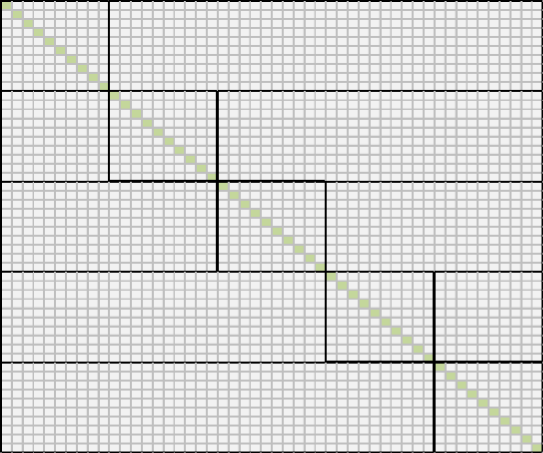
\includegraphics[scale=0.35]{fronty.png}\hspace*{\fill}
\end{frame}

\subsection{Równoległy wariant metody Gaussa}
\begin{frame}
\frametitle{Algorytm}
\framesubtitle{Równoległy wariant metody Gaussa}

\begin{itemize}[<+->]
\item Operacje elementarne na macierzach
\begin{itemize}
\item Mnożenie i dodawanie wierszy
\item Zamiana wierszy
\end{itemize}
\item Koncepcja mapy
\begin{itemize}
\item Uniknięcie kosztownej, fizycznej zamiany wierszy
\end{itemize}
\item Przywracanie formy macierzy schodkowej
	\begin{itemize}
	\item Unikalny pierwszy wyraz niezerowy w wierszu
	\item Mapa:
		\begin{itemize}
		\item Pozwala na szybką weryfikację unikalności
		\item Informuje względem którego wiersza prowadzić eliminację
		\end{itemize}
	\end{itemize}
\end{itemize}
\end{frame}

\subsection{Przykład}

\begin{frame}
\frametitle{Algorytm}
\framesubtitle{Równoległy wariant metody Gaussa}
\hfill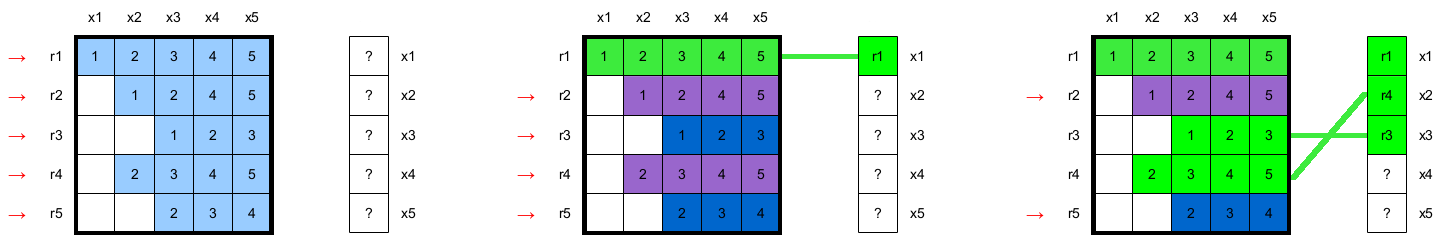
\includegraphics[scale=0.3]{faza1_initialSelections.png}\hspace*{\fill}
\end{frame}


\begin{frame}
\frametitle{Algorytm}
\framesubtitle{Równoległy wariant metody Gaussa}
\hfill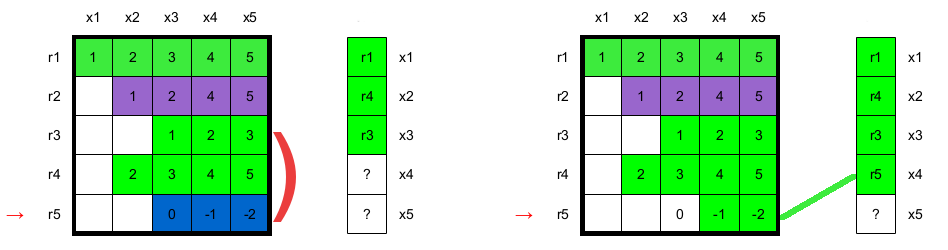
\includegraphics[scale=0.45]{faza2a_conflictResolution.png}\hspace*{\fill}
\end{frame}

\begin{frame}
\frametitle{Algorytm}
\framesubtitle{Równoległy wariant metody Gaussa}
\hfill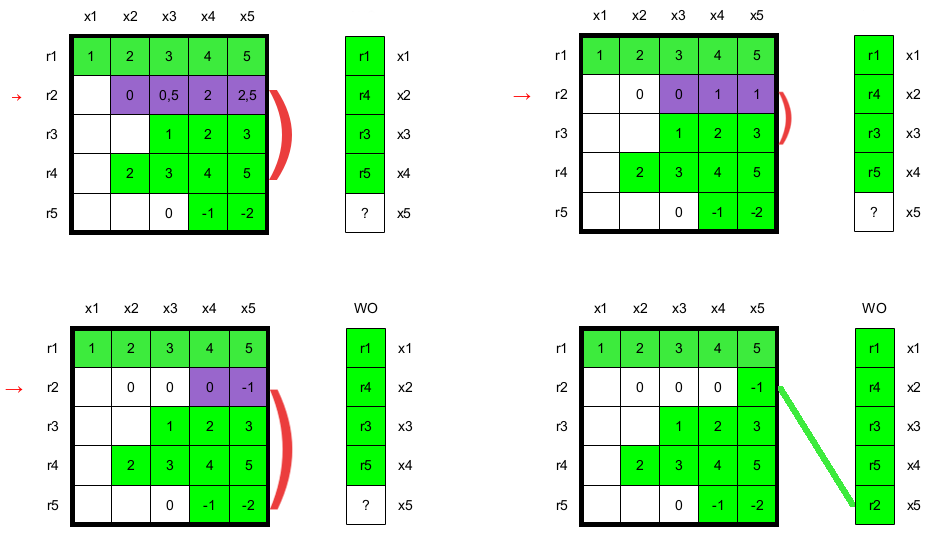
\includegraphics[scale=0.45]{faza2b_conflictResolution.png}\hspace*{\fill}
\end{frame}

\section{Realizacja projektu}
\subsection{Problemy równoległości masowej}

\begin{frame}
\frametitle{Realizacja projektu}
\framesubtitle{Problemy równoległości masowej}
\begin{itemize}[<+->]
\item Wewnątrz części macierzy (frontu) wydzielane są grupy robocze
	\begin{itemize}
	\item Wynika to z architektury urządzeń obliczeniowych
	\end{itemize}
\item Przedstawiony wcześniej algorytm działa w obrębie grupy
	\begin{itemize}
	\item Pewność, iż nie ma konfliktujących wierszy w obrębie grupy
	\item Co z konfliktami w obrębie całego frontu?
	\item Co z konfliktami w obrębie całej macierzy?
	\end{itemize}
\item Rozwiązanie
	\begin{itemize}
	\item Dodatkowy kernel na urządzeniu obliczeniowym
	\item Dodatkowa faza przetwarzania na CPU
	\end{itemize}
\end{itemize}
\end{frame}

\subsection{Przykład funkcjonowania jednego frontu}

\begin{frame}
\frametitle{Realizacja projektu}
\framesubtitle{Przykład funkcjonowania jednego frontu}
\begin{columns}[t] % contents are top vertically aligned
     \begin{column}[T]{5cm} % each column can also be its own environment
     \begin{itemize}
		\item Istnieje tyle lokalnych map, ile grup roboczych
		\item Przynależność map oznaczono kolorem
     \end{itemize}
     \end{column}
     \begin{column}[T]{7cm} % alternative top-align that's better for graphics
		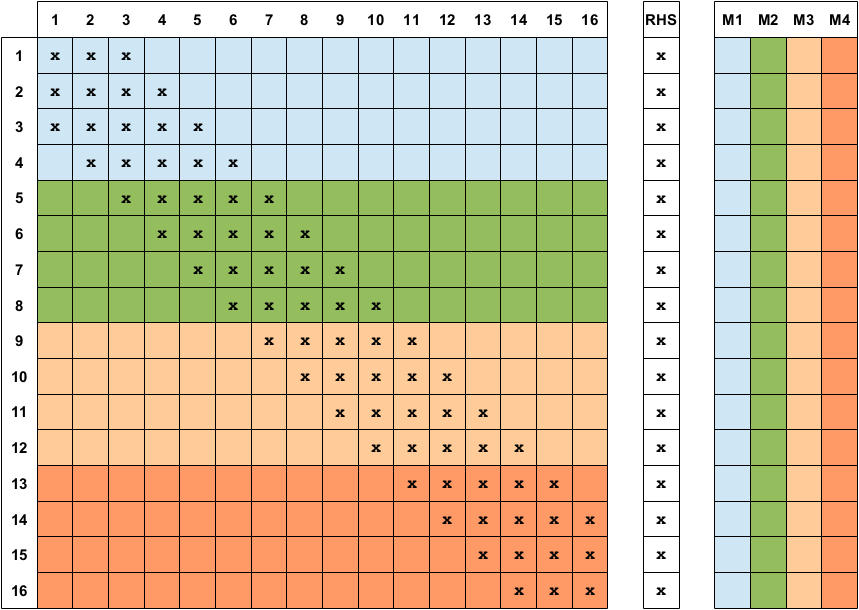
\includegraphics[scale=0.3]{frame0.jpg}
     \end{column}
     \end{columns}
\end{frame}

\begin{frame}
\frametitle{Realizacja projektu}
\framesubtitle{Przykład funkcjonowania jednego frontu}
\begin{columns}[t] % contents are top vertically aligned
     \begin{column}[T]{5cm} % each column can also be its own environment
     \begin{itemize}
		\item Konflikty w obrębie grup zostały rozwiązane
		\item\alert Istnieją konflikty w obrębie frontu
     \end{itemize}
     \end{column}
     \begin{column}[T]{7cm} % alternative top-align that's better for graphics
		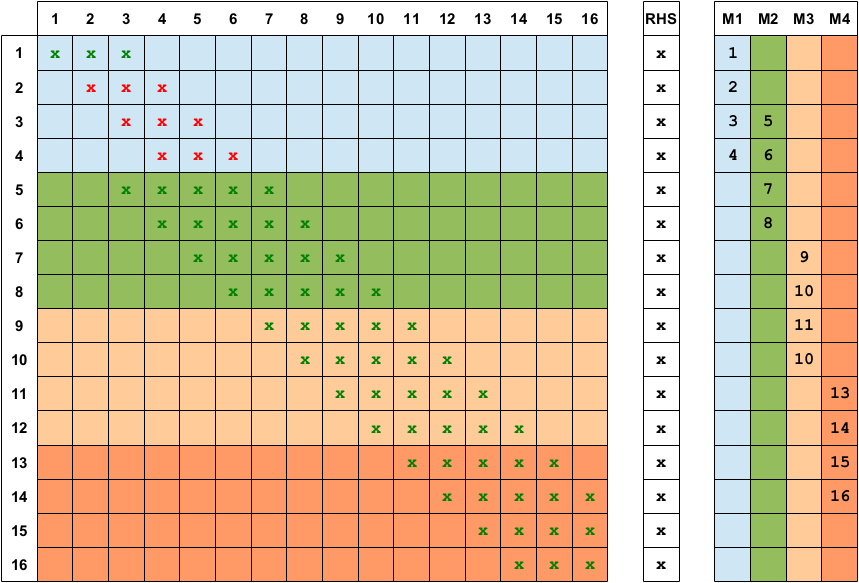
\includegraphics[scale=0.3]{frame1.jpg}
     \end{column}
     \end{columns}
\end{frame}

\begin{frame}
\frametitle{Realizacja projektu}
\framesubtitle{Przykład funkcjonowania jednego frontu}
\begin{columns}[t] % contents are top vertically aligned
     \begin{column}[T]{5cm} % each column can also be its own environment
     \begin{itemize}
		\item Konflikty w obrębie frontu zostały rozwiązane
		\item Poczyniono zmiany: czy nie powstały nowe konflikty w obrębie grup roboczych?
     \end{itemize}
     \end{column}
     \begin{column}[T]{7cm} % alternative top-align that's better for graphics
		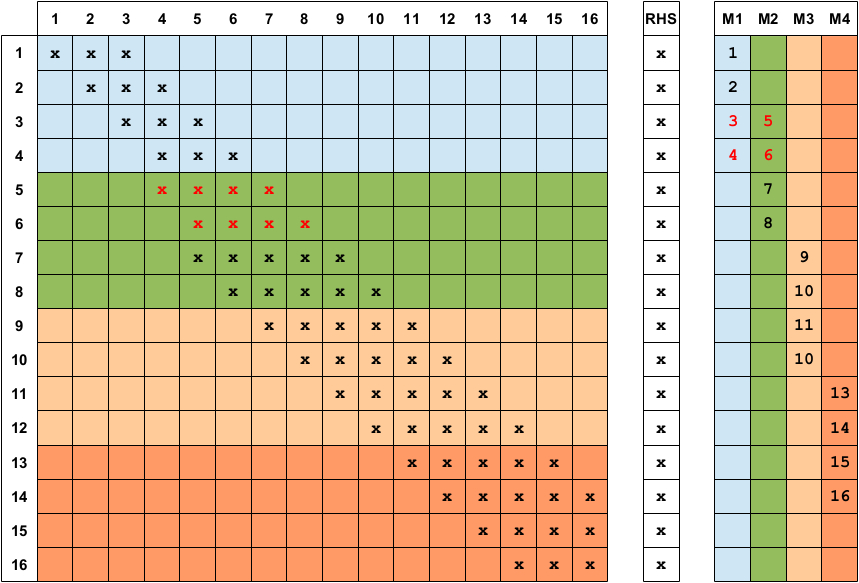
\includegraphics[scale=0.3]{frame2.jpg}
     \end{column}
     \end{columns}
\end{frame}

\begin{frame}
\frametitle{Realizacja projektu}
\framesubtitle{Przykład funkcjonowania jednego frontu}
\begin{columns}[t] % contents are top vertically aligned
     \begin{column}[T]{5cm} % each column can also be its own environment
     \begin{itemize}
		\item Kernele wykonywane naprzemiennie dopóki drugi nie zgłosi zerowej ilości wykonanych operacji
		\item Kiedy wszystkie części skończą przetwarzanie analogiczna operacja jest powtarzana po stronie hosta
     \end{itemize}
     \end{column}
     \begin{column}[T]{7cm} % alternative top-align that's better for graphics
		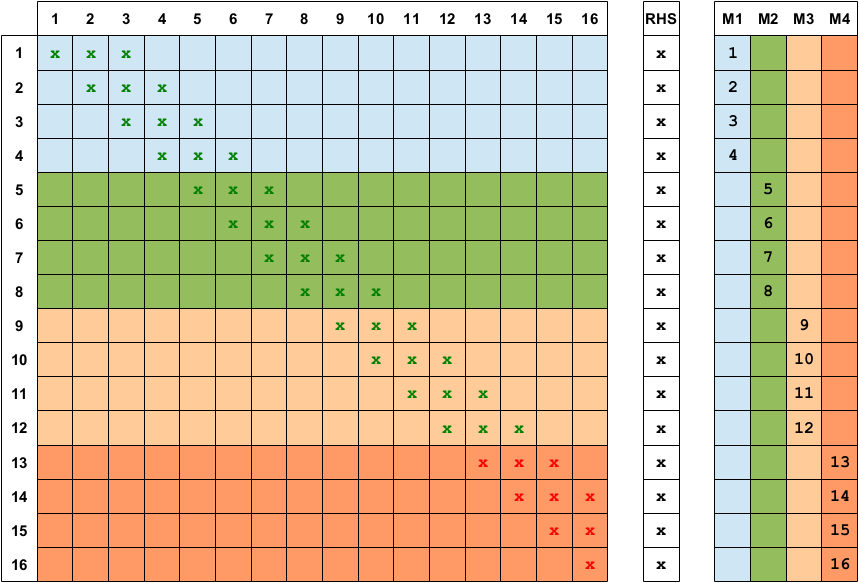
\includegraphics[scale=0.3]{frame9.jpg}
     \end{column}
     \end{columns}
\end{frame}

\subsection{Paradygmat czarnej skrzynki}

\begin{frame}
\frametitle{Realizacja projektu}
\framesubtitle{Paradygmat czarnej skrzynki}

\begin{itemize}[<+->]
	\item Projekt zrealizowany jako biblioteka nagłówkowa
	\begin{itemize}
		\item Nie wymaga dodatkowej kompilacji i linkowania ze strony użytkownika
		\item Kompiluje się razem z kodem użytkownika
	\end{itemize}
	\item Nie wymaga informacji o rozwiązywanym problemie
	\begin{itemize}
		\item Nie integruje się z siatką MES
		\item Może rozwiązywać dowolne problemy postawione jako układ równań liniowych
	\end{itemize}
	\item Eksponuje wygodny interfejs
		\begin{itemize}
		\item Dostarczany jest jeden wielofunkcyjny obiekt
		\item Dostarczane są funkcje konwersji z macierzy użytkownika do wewnętrznych macierzy solwera
		\end{itemize}
	\item Pozwala na wymianę kerneli już po skompilowaniu kodukur
\end{itemize}

\end{frame}

\section{Badania wydajności}

\subsection{Optymalna liczba wątków dla badanych urządzeń}

\begin{frame}
\frametitle{Badania wydajności}
\framesubtitle{Optymalna liczba wątków dla badanych urządzeń}
\hfill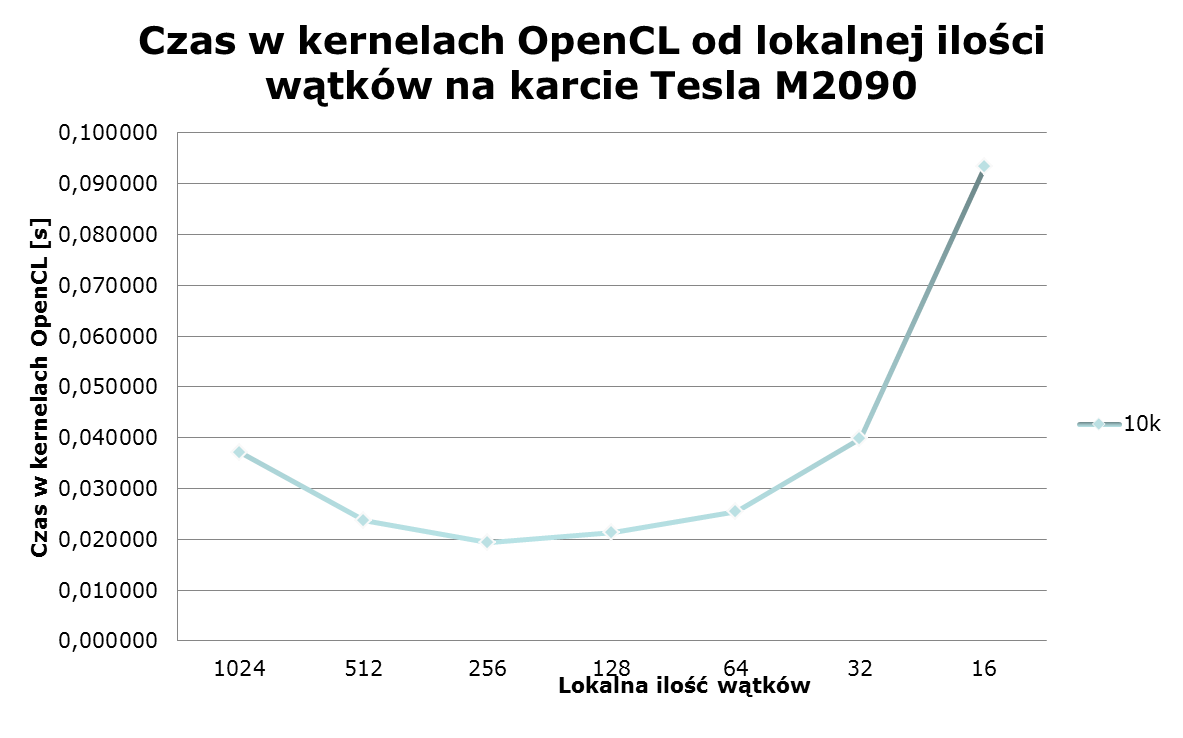
\includegraphics[scale=0.45]{czas1.png}\hspace*{\fill}
\end{frame}

\begin{frame}
\frametitle{Badania wydajności}
\framesubtitle{Optymalna liczba wątków dla badanych urządzeń}
\hfill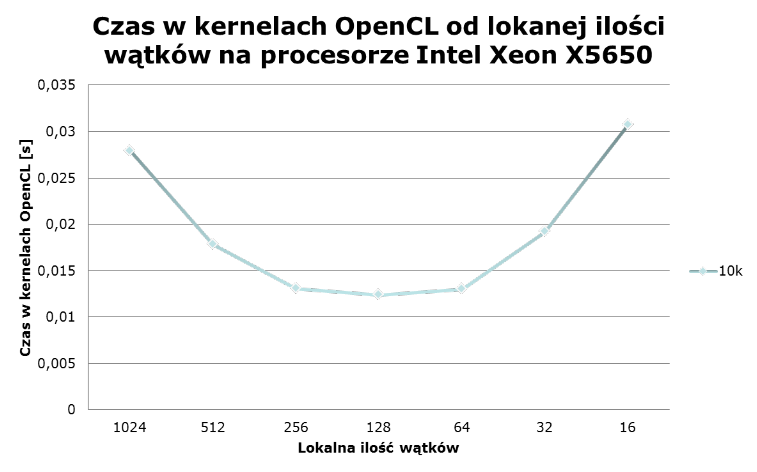
\includegraphics[scale=0.35]{czas2.png}\hspace*{\fill}
\end{frame}

\subsection{Przyspieszenie w zależności od globalnej ilości wątków}

\begin{frame}
\frametitle{Badania wydajności}
\framesubtitle{Przyspieszenie w zależności od globalnej ilości wątków}
\hfill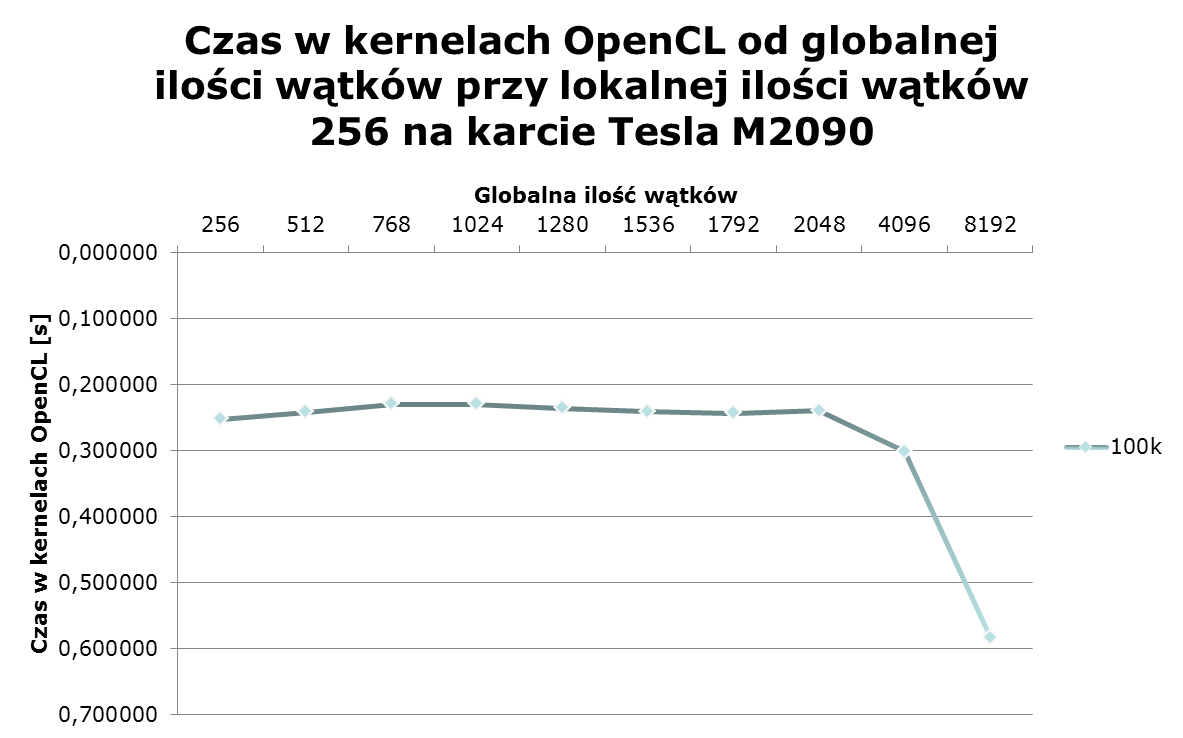
\includegraphics[scale=0.45]{czas3.png}\hspace*{\fill}
\end{frame}

\begin{frame}
\frametitle{Badania wydajności}
\framesubtitle{Przyspieszenie w zależności od globalnej ilości wątków}
\hfill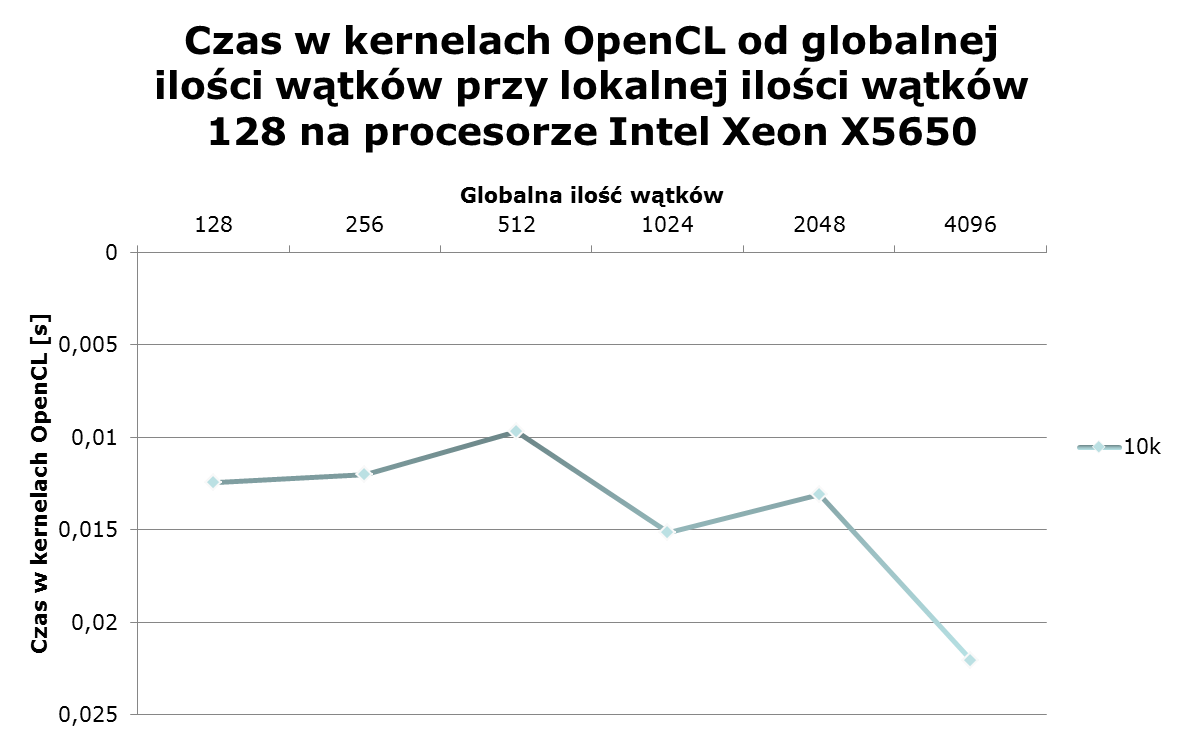
\includegraphics[scale=0.45]{czas4.png}\hspace*{\fill}
\end{frame}

\subsection{Skalowalność}

\begin{frame}
\frametitle{Badania wydajności}
\framesubtitle{Skalowalność}
\hfill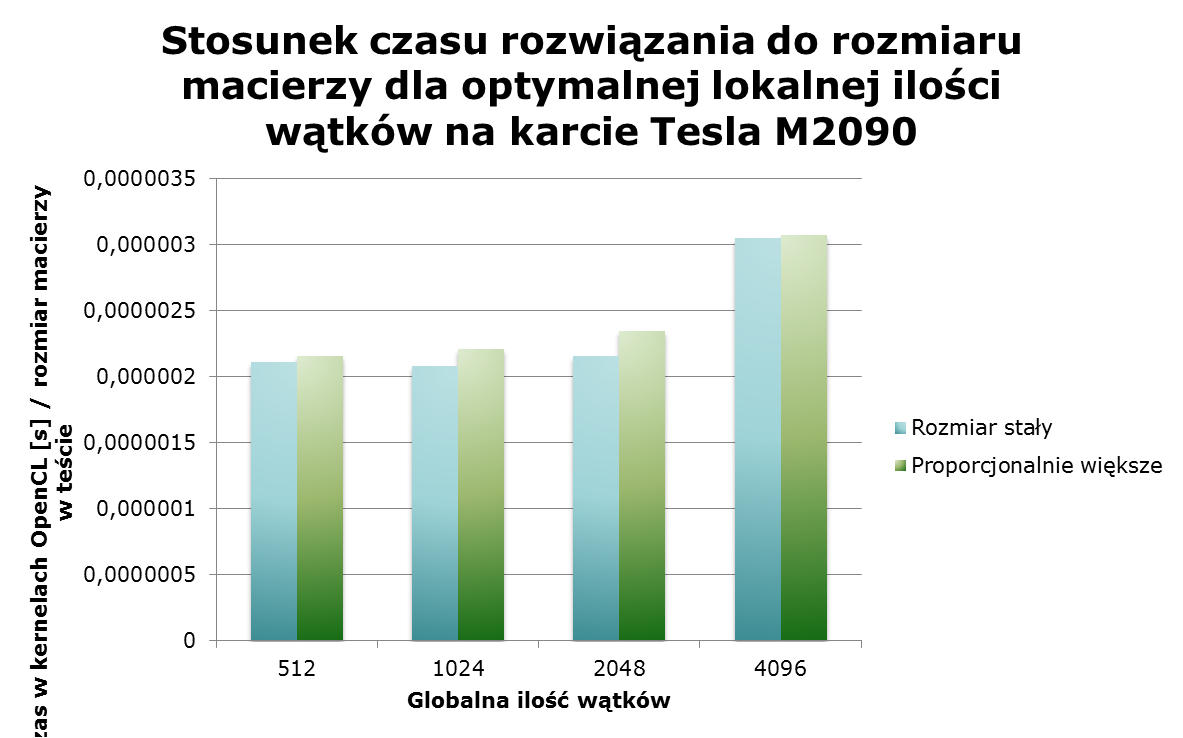
\includegraphics[scale=0.45]{czas5.png}\hspace*{\fill}
\end{frame}

\begin{frame}
\frametitle{Badania wydajności}
\framesubtitle{Skalowalność}
\hfill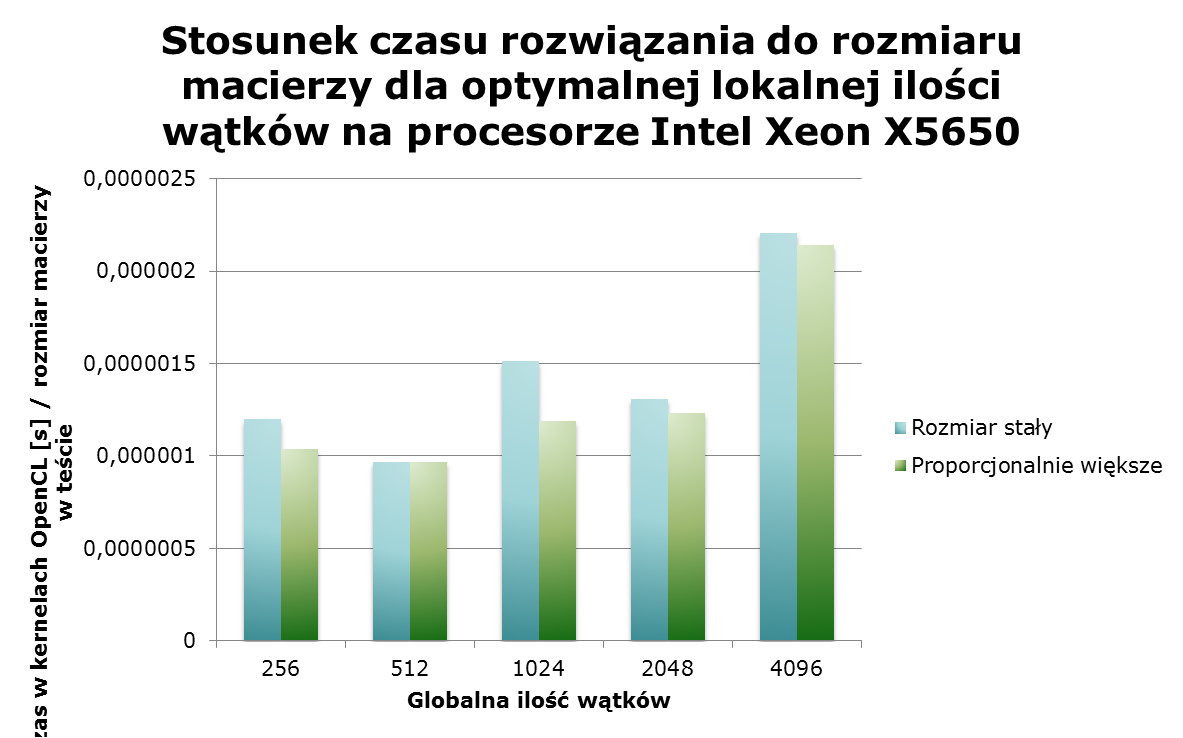
\includegraphics[scale=0.45]{czas6.png}\hspace*{\fill}
\end{frame}

\section{Podsumowanie projektu}
\subsection{Wykonana praca}

\begin{frame}
\frametitle{Podsumowanie projektu}
\framesubtitle{Wykonana praca}
\begin{itemize}

\item Stworzono równoległy algorytm rozwiązywania układów równań w oparciu o metodę Gaussa
\item Zaproponowano masowo równoległy, frontalny solwer MES z wykorzystaniem technologii OpenCL
\item Oprogramowanie powstało zgodnie z paradygmatem czarnej skrzynki
	\begin{itemize}
	\item Łatwe w przeniesieniu między systemami operacyjnymi i urządzeniami
	\item Łatwe w implementacji w innych projektach
	\end{itemize}
\end{itemize}
\end{frame}

\subsection{Kontynuacja projektu}

\begin{frame}
\frametitle{Podsumowanie projektu}
\framesubtitle{Kontynuacja projektu}
\begin{itemize}
\item Kontynuowana jest praca nad projektem
	\begin{itemize}
	\item Wykorzystanie wielu urządzeń na jednym węźle obliczeniowym
	\item Rozproszenie obliczeń na wiele węzłów
	\end{itemize}
\end{itemize}
\end{frame}

\end{document}

